\documentclass[12pt,letterpaper]{article}
\usepackage{fullpage, lastpage, fancyhdr, enumerate}
\usepackage[top=2cm, bottom=4.5cm, left=2.5cm, right=2.5cm]{geometry}
\usepackage{amsmath,amsthm,amsfonts,amssymb,amscd}
\usepackage{mathrsfs, listings, hyperref}
\usepackage{xcolor, graphicx}
\graphicspath{{./images}}

\setlength{\parindent}{0.0in}
\setlength{\parskip}{0.05in}

\title{A Bayesian Approach to Hit Probability}
\author{Matthew Bernstein}

\begin{document}

\maketitle

\section*{Introduction}
Expected Batting Average ($xBA$) is an attempt to quantify a hitter’s batting average using only the batted balls launch angle and exit velocity. Each batted ball is assigned an expected batting average based on how often comparable batted balls have become hits . This attempts to remove factors such as weather and defensive ability to isolate hitter skill and can be an important tool in assessing hitter ability.

The current xBA model is based solely on empirical data. This provides good predictive qualities but comes with some notable drawbacks. First, due to the reliance on historical data, access to that data is necessary to calculate it for future batted balls. This method also does not delineate between balls hit in different environments or different “eras”. The 2023 MLB season brought rule changes, notably banning the defensive shift, that could cause future batted balls to be hits while previous ones would not. Finally, Statcast only uses two elements of a batted ball for predictions. Other features, such as spray angle and distance, could improve predictive power. 

A model to determine the probability of any batted ball to be a hit would be a more accessible way to determine if the $xBA$ for a particular hitter. It could also be trained on specific subsets of data, such as from a specific park or time period, to focus the model for specific situations. 

\section*{Statcast Baseline}
The dataset includes all batted ball events from June 2022, with all sacrifice bunts, hits, and flyballs removed. In order to compare the model, a Statcast classification of every batted ball was calculated using the following formula:
\begin{align*}
    Hit =
        \begin{cases}
            1 & \text{if } xBA \ge 0.500\\
            0 & \text{if } xBA < 0.500
        \end{cases}
\end{align*}

The data was partitioned randomly into a training and test set on a 70/30 split. In addition to Statcast classifications, an additional control of predicting 0, or "out", everytime was used as a reference. Figure \ref{fig:baseline_cm} shows the confustion matrix for Statcast classifications on the training set. Table \ref{tab:baseline_acc} shows accuracy methods of the baseline methods and Figure \ref{fig:baseline_roc} superimposes the ROC curves of the two baseline methods. 

\begin{figure}[!htb]
    \centering
    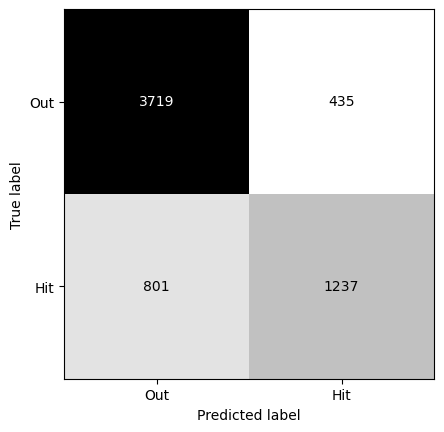
\includegraphics[width=0.5\textwidth]{baseline_cm}
    \caption{Confusion matrix for Statcast classifications}
    \label{fig:baseline_cm}
\end{figure}

\begin{table}[!htb]
    \centering
    \begin{tabular}{|r|c|c|c|c|}
        \hline
        & Accuracy & Sensitivity & Specificity & F1 Score \\ \hline
        Statcast & 0.800 & 0.607 & 0.895 & 0.667 \\ \hline
        Alaways Out & 0.671 & 0.0000 & 1.000 & 0.000 \\ \hline
    \end{tabular}
    \caption{Scores for baseline models}
    \label{tab:baseline_acc}
\end{table}

\begin{figure}[!htb]
    \centering
    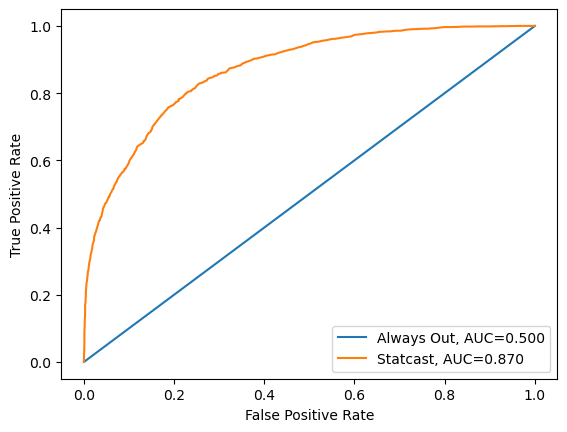
\includegraphics[width=0.5\textwidth]{baseline_roc}
    \caption{ROC curve of baseline methods}
    \label{fig:baseline_roc}
\end{figure}

The Statcast classifications are quite accurate on the whole, but struggles at successfully predicting hits. Since around 2/3 of all batted balls are outs, predicting a batted ball as an out should be the default classification. 

\end{document}